\documentclass[final,5p]{elsarticle}

% \documentclass[preprint,12pt]{elsarticle}

%% Use the option review to obtain double line spacing
%% \documentclass[authoryear,preprint,review,12pt]{elsarticle}

%% Use the options 1p,twocolumn; 3p; 3p,twocolumn; 5p; or 5p,twocolumn
%% for a journal layout:
% \documentclass[final,1p,times]{elsarticle}
%% \documentclass[final,1p,times,twocolumn]{elsarticle}
% \documentclass[final,3p,times]{elsarticle}
%% \documentclass[final,3p,times,twocolumn]{elsarticle}
% \documentclass[final,5p,times]{elsarticle}
%% \documentclass[final,5p,times,twocolumn]{elsarticle}
\usepackage[portuguese]{babel}

%% For including figures, graphicx.sty has been loaded in
%% elsarticle.cls. If you prefer to use the old commands
%% please give \usepackage{epsfig}

%% The amssymb package provides various useful mathematical symbols
\usepackage{amssymb}
\usepackage{amsmath}
\usepackage{multirow}
\usepackage{tabularx}
\usepackage{booktabs}
\usepackage{tablefootnote}

\usepackage{pgfplots}
\pgfplotsset{compat=1.18}
\usepgfplotslibrary{statistics}
\usepackage{pgfplotstable}

\usepackage{placeins}
\usepackage{hyperref}
\numberwithin{equation}{section}

\usepackage{algorithm}
\usepackage[noEnd=true, indLines=true]{algpseudocodex}
\algrenewcommand\algorithmicrequire{\textbf{Entrada:}}
\algrenewcommand\algorithmicwhile{\textbf{Enquanto}}
\algrenewcommand\algorithmicrepeat{\textbf{Repete}}
\algrenewcommand\algorithmicuntil{\textbf{Até}}
\algrenewcommand\algorithmicif{\textbf{Se}}
\algrenewcommand\algorithmicthen{\textbf{então}}
\algrenewcommand\algorithmicelse{\textbf{Caso contrário}}
\algrenewcommand\algorithmicensure{\textbf{Objetivo:}}
\algrenewcommand\algorithmicreturn{\textbf{Retorna:}}
\algrenewcommand\algorithmicdo{\textbf{faça}}
\algrenewcommand\algorithmicforall{\textbf{Para todos}}
\algnewcommand{\LineComment}[1]{\State \(\triangleright\) \textcolor{black!50}{\emph{#1}}}

\newcommand*{\squareb}{\textcolor{black}{\rule{0.5em}{0.5em}}}
\newcommand*{\squareg}{\textcolor{gray}{\rule{0.5em}{0.5em}}}

\graphicspath{ {./png/} }

% \usepackage[fleqn]{nccmath}
% \usepackage{multicol}


%=========== Gloabal Tikz settings
% \pgfplotsset{compat=newest}
% \usetikzlibrary{math}
% \pgfplotsset{
%     height = 10cm,
%     width = 10cm,
%     tick pos = left,
%     legend style={at={(0.98,0.30)}, anchor=east},
%     legend cell align=left,
%     }
%  \pgfkeys{
%     /pgf/number format/.cd,
%     fixed,
%     precision = 1,
%     set thousands separator = {}
% }

%% The amsthm package provides extended theorem environments
%% \usepackage{amsthm}

%% The lineno packages adds line numbers. Start line numbering with
%% \begin{linenumbers}, end it with \end{linenumbers}. Or switch it on
%% for the whole article with \linenumbers.
%% \usepackage{lineno}

\usepackage{listings}
\usepackage{xcolor}

\definecolor{codegreen}{rgb}{0,0.6,0}
\definecolor{codegray}{rgb}{0.5,0.5,0.5}
\definecolor{codepurple}{rgb}{0.58,0,0.82}
\definecolor{backcolour}{rgb}{0.98,0.98,0.98}

\lstdefinestyle{mystyle}{
    backgroundcolor=\color{backcolour},
    commentstyle=\color{codegreen},
    keywordstyle=\color{magenta},
    numberstyle=\tiny\color{codegray},
    stringstyle=\color{codepurple},
    basicstyle=\ttfamily\footnotesize,
    breakatwhitespace=false,
    breaklines=true,
    captionpos=b,
    keepspaces=true,
    numbers=left,
    numbersep=5pt,
    showspaces=false,
    showstringspaces=false,
    showtabs=false,
    tabsize=2
}

\lstset{style=mystyle}

% \journal{Nuclear Physics B}

\begin{document}

\begin{frontmatter}

%% Title, authors and addresses

%% use the tnoteref command within \title for footnotes;
%% use the tnotetext command for theassociated footnote;
%% use the fnref command within \author or \address for footnotes;
%% use the fntext command for theassociated footnote;
%% use the corref command within \author for corresponding author footnotes;
%% use the cortext command for theassociated footnote;
%% use the ead command for the email address,
%% and the form \ead[url] for the home page:
%% \title{Title\tnoteref{label1}}
%% \tnotetext[label1]{}
%% \author{Name\corref{cor1}\fnref{label2}}
%% \ead{email address}
%% \ead[url]{home page}
%% \fntext[label2]{}
%% \cortext[cor1]{}
%% \affiliation{organization={},
%%             addressline={},
%%             city={},
%%             postcode={},
%%             state={},
%%             country={}}
%% \fntext[label3]{}

\title{Resolução de Sistema de Equações Lineares de Matrizes Pentadiagonais com Redes Neurais Convolucionais\tnoteref{label_title}}
\tnotetext[label_title]{Projeto final como parte dos requisitos da disciplina IA048: Aprendizado de Máquina.}

%% use optional labels to link authors explicitly to addresses:
%% \author[label1,label2]{}
%% \affiliation[label1]{organization={},
%%             addressline={},
%%             city={},
%%             postcode={},
%%             state={},
%%             country={}}
%%
%% \affiliation[label2]{organization={},
%%             addressline={},
%%             city={},
%%             postcode={},
%%             state={},
%%             country={}}

\author[label1]{Tiago C A Amorim (RA: 100675)}
\affiliation[label1]{organization={Doutorando no Departamento de Engenharia de Petróleo da Faculdade de Engenharia Mecânica, UNICAMP},
            city={Campinas},
            state={SP},
            country={Brasil}}

\author[label2]{Taylon L C Martins (RA: 177379)}
\affiliation[label2]{organization={Aluno especial, UNICAMP},
            city={Campinas},
            state={SP},
            country={Brasil}}


% \begin{abstract}

%     xxxxxxx

% \end{abstract}


%%Graphical abstract
% \begin{graphicalabstract}
%\includegraphics{grabs}
% \end{graphicalabstract}

%%Research highlights
% \begin{highlights}
% \item Research highlight 1
% \item Research highlight 2
% \end{highlights}

\begin{keyword}
    Rede Neurais Convolucionais \sep Sistemas de Equações Lineares
%% keywords here, in the form: keyword \sep keyword

%% PACS codes here, in the form: \PACS code \sep code

%% MSC codes here, in the form: \MSC code \sep code
%% or \MSC[2008] code \sep code (2000 is the default)

\end{keyword}

\end{frontmatter}

%% main text
\section{Introdução}

     O método das diferenças finitas é utilizado para resolver diferentes problemas físicos que podem ser descritos como equações diferenciais. O método se baseia na aproximação das derivadas por diferenças finitas (exemplos em \ref{eq:diffin}). O domínio espaço-temporal é discretizado e a solução das equações diferenciais é aproximada nos nós desta malha \cite{causon2010introductory}. O problema então é transformado em uma série de equações não-lineares, que usualmente são resolvidas por métodos numéricos, como o método de Newton-Raphson \cite{burden2016analise}.

    \begin{subequations}
        \begin{align}
            \frac{\partial u(x)}{\partial x} &\approx \frac{u(x+h) - u(x-h)}{2h} \\
            \frac{\partial^2 u(x)}{\partial x^2} &\approx \frac{u(x+h) - 2u(x) + u(x-h)}{h^2}
        \end{align}
        \label{eq:diffin}
    \end{subequations}

    É usual utilizar aproximações de derivada que utilizam os valores da função do nó e seus vizinhos diretos. Em problemas bidimensionais com malhas regulares (Figura \ref{fig:esquematico}) esta escolha leva a sistemas de equações com matrizes pentadiagonais (exemplo para uma malha $n_i$,$n_j$ em \ref{eq:sistema}). Cada equação não-linear tem termos associados a um dos nós (i,j) e seus quatro vizinhos: (i-1,j), (i+1,j), (i,j-1) e (i,j+1). A resolução numérica deste sistema de equações não-lineares usualmente está associada a métodos iterativos, em que novas equações lineares são resolvidas. Desta forma, a resolução do problema original está associada à solução de um significativo número de sistemas de equações lineares com matriz pentadiagonal.

    A proposta deste trabalho é avaliar a possibilidade de utilizar uma rede convolucional para resolver este tipo de sistema de equações lineares.

    \begin{figure}
    \begin{center}
        \begin{tabular}{c|c|c|c|c}
            & &  & & \\
            \hline
            & & (i,j-1) & & \\
            \hline
            & (i-1,j) & \textbf{(i,j)} & (i+1,j) & \\
            \hline
            & & (i,j+1) & & \\
            \hline
            & &  & & \\
        \end{tabular}
        \caption{Esquemático de uma malha regular, com destaque para a célula (i,j) e seus vizinhos.}
        \label{fig:esquematico}
    \end{center}
    \end{figure}

    \begin{figure*}
        \begin{equation}
            \overbrace{
            \begin{bmatrix}
                a^0_1    & a^1_1    & 0       & \ldots  & 0      & a^{n_i}_1   & 0       &         & \ldots    &  0      \\
                a^{-1}_2   & a^0_2    & a^1_2 & 0       & \ldots & 0         & a^{n_i}_2 & 0       & \ldots    &  0      \\
                0          & a^{-1}_3   & a^0_3 & a^1_3 & 0      & \ldots    & 0       & a^{n_i}_3 & \ldots    & 0       \\
                \vdots     &            & \ddots  & \ddots  & \ddots &           &         &         & \ddots    & \vdots  \\
                0          & \ldots     & 0      & a^{-n_i}_{n_in_j-2}  & 0       & \ldots  & a^{-1}_{n_in_j-2}  & a^0_{n_in_j-2} & a^1_{n_in_j-2} & 0 \\
                0          & \ldots     &         & 0      & a^{-n_i}_{n_in_j-1}  & 0       & \ldots  & a^{-1}_{n_in_j-1}  & a^0_{n_in_j-1} & a^1_{n_in_j-1} \\
                0          & \ldots     &         &         & 0      & a^{-n_i}_{n_in_j}  & 0       & \ldots  & a^{-1}_{n_in_j}  & a^0_{n_in_j} \\
            \end{bmatrix}}^\textbf{A}
            \overbrace{
            \begin{bmatrix}
                x_1 \\
                x_2 \\
                x_3 \\
                \vdots \\
                x_{n_in_j-2} \\
                x_{n_in_j-1} \\
                x_{n_in_j} \\
            \end{bmatrix}}^\textbf{x}
            =
            \overbrace{
            \begin{bmatrix}
                b_1 \\
                b_2 \\
                b_3 \\
                \vdots \\
                b_{n_in_j-2} \\
                b_{n_in_j-1} \\
                b_{n_in_j} \\
            \end{bmatrix}}^\textbf{b}
            \label{eq:sistema}
        \end{equation}
    \end{figure*}


\section{Trabalhos Correlatos}

    Não foram encontrados muitos trabalhos com foco na resolução de sistemas de equações lineares com redes neurais. Dentre os trabalhos encontrados, duas formas distintas de resolução do problema foram propostas. A primeira vertente é resolver o sistema de equações lineares junto com o treinamento da rede \cite{cichocki1992neural}. Uma aplicação interessante desta proposta é o de resolver sistemas de grande dimensão, que possivelmente não cabem na memória disponível, e usar a rede para aprender um mapeamento que aproxima a resposta \cite{gu2023deep}.

    Uma segunda vertente é a de treinar uma rede neural com base em vários exemplos de sistemas de equações a resolver. A rede treinada é utilizada para resolver novos sistemas de equações. Uma proposta focou na solução de sistemas tridiagonais \cite{jiang2023neural}, utilizando uma série de camadas densas seguidas por conexões residuais. Um outro trabalho \cite{kontolati2024learning} foca na solução de problemas físicos associados a equações diferenciais. Este trabalho tenta primeiro encontrar uma representação densa dos dados de entrada por meio de uma rede \emph{autoenconder}. Posteriormente a representação densa de cada amostra passa por uma outra rede neural que busca resolver o problema.

    A proposta estudada neste projeto segue a segunda vertente. Ao contrário das demais aplicações, onde foram utilizadas camadas densas, foi feita a opção de utilizar camadas convolucionais para que a arquitetura da rede seja agnóstica à discretização do problema (tamanho da malha).

\section{Codificação do Sistema Linear}

    O objetivo da rede é resolver um problema do tipo $\textbf{Ax}=\textbf{b}$. Cada amostra da base de dados são os valores das diagonais da matriz $\textbf{A}$ e o vetor $\textbf{b}$, e a saída pretendida são os valores de $\textbf{x}$. É possível dividir as linhas da matriz $\textbf{A}$ e o vetor $\textbf{b}$ pelos valores da diagonal principal de $\textbf{A}$. Esta operação não muda o vetor $\textbf{x}$ que resolve o sistema. Desta forma na nova matriz pentadiagonal todos os valores da diagonal principal são iguais à unidade. Como todas amostras tem estes mesmos valores, não é necessário apresentar estes valores à rede.

    Os dados são organizados em forma de tensor 2D, à semelhança de uma imagem com ($n_i$,$n_j$) pixels. Seguindo a notação utilizada em \ref{eq:sistema}, os \emph{canais} desta imagem correspondem aos valores das diagonais $-n_i$, $-1$, $1$ e $n_i$, e os valores de $\textbf{b}$. Cada um destes vetores é ajustado para que os termos fiquem na posição (i,j) correspondente ao nó associado ao valor. Como as diagonais tem $n_i(n_j-1)$ e $(n_i-1)n_j$ valores, uma linha ou coluna do tensor associado tem valores nulos.

    A saída pretendida, o vetor $\textbf{x}$, também é formatada como um tensor 2D. A saída tem apenas um canal. Desta forma, a rede neural recebe uma \emph{imagem} ($n_i$,$n_j$) com 5 canais e deve gerar uma imagem de mesmo tamanho com um canal.

\section{Arquitetura e Treinamento}

    Como as \emph{resoluções} dos dados de entrada e saída da rede são as mesmas, optou-se por utilizar apenas camadas que mantém este tamanho. A rede é composta por (Figura \ref{fig:arquitetura}):

    \begin{enumerate}
        \item Camada convolucional com \emph{kernel}=1x1: passa de 5 para $n_{lat}$ o número de canais (ativação: ReLu).
        \item $N$ camadas convolucionais com \emph{kernel}=3x3 e \emph{padding}=1 (ativação: ReLu).
        \item Camada convolucional com \emph{kernel}=1x1: passa de $n_{lat}$ para um canal.
    \end{enumerate}

    \begin{figure}[hbt!]
        \centering
        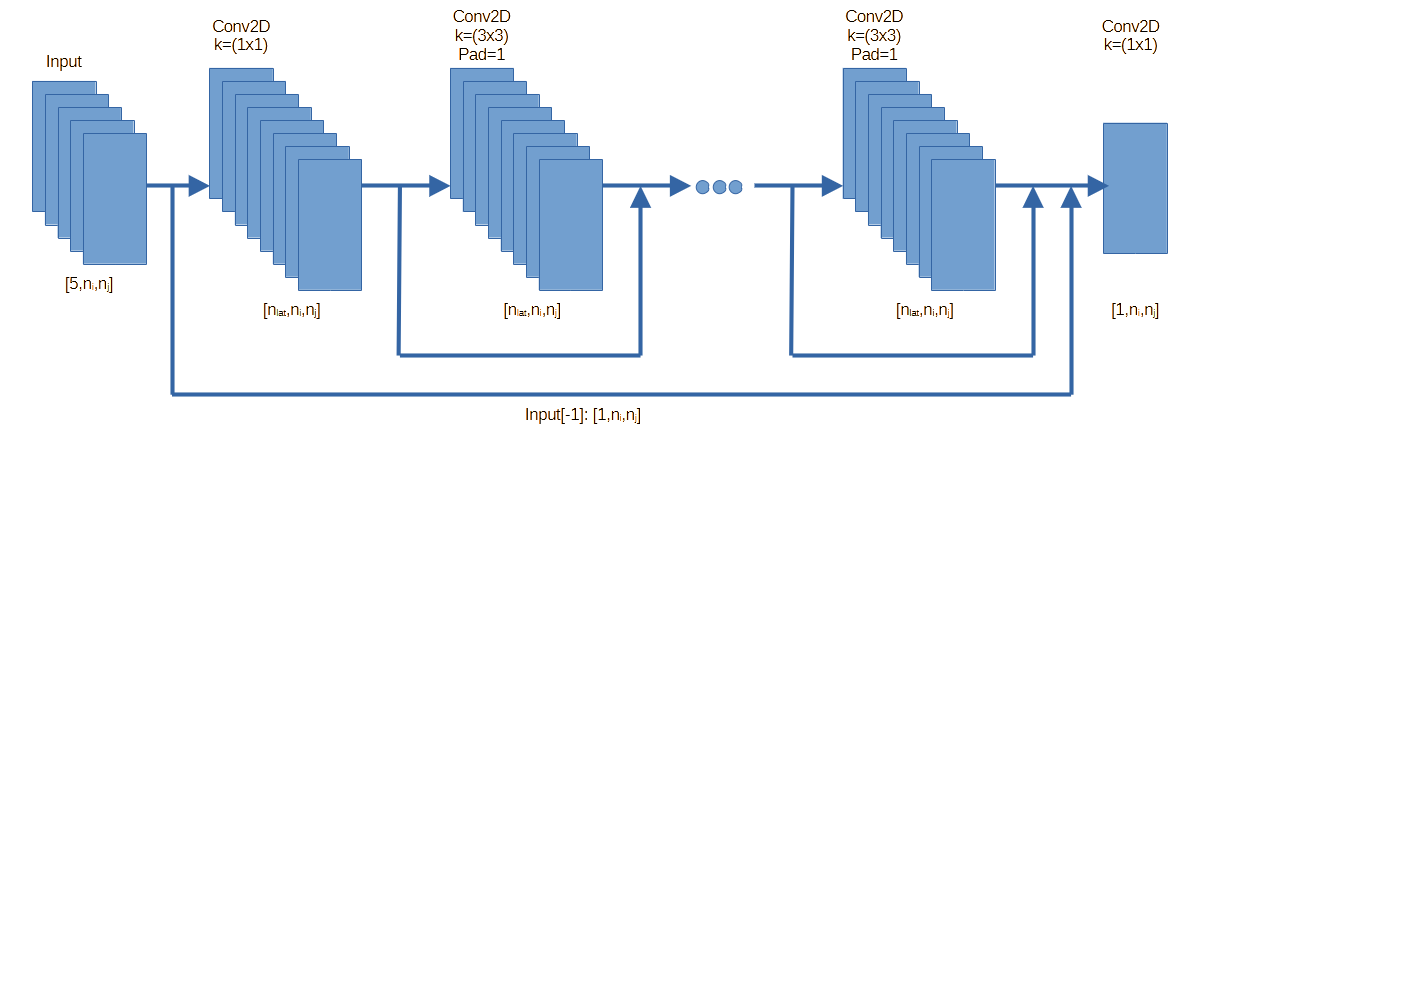
\includegraphics[width=0.95\columnwidth, trim={0cm 7.8cm 1cm 0cm}, clip]{./fig/NN.png}
        \caption{Arquitetura geral da rede neural proposta.}\label{fig:arquitetura}
    \end{figure}

    A ligação direta entre os dados de entrada e a saída é dos valores do vetor $\textbf{b}$ (último \emph{canal} de cada amostra).

    A classe que constrói a rede neural tem diferentes opções de configuração, de forma a poder ser feita uma otimização destes hiperparâmetros. Entre as opções de arquitetura, existe a possibilidade de trocar as camadas convolucionais com \emph{kernel}=3x3 por blocos \textbf{Inception} (Figura \ref{fig:inception}).

    \begin{figure}[hbt!]
        \centering
        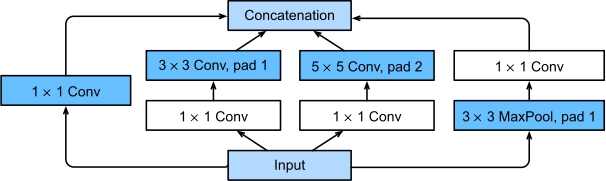
\includegraphics[width=0.95\columnwidth]{./fig/inception.png}
        \caption{Bloco Inception. (Fonte: \cite{zhang2021dive})}\label{fig:inception}
    \end{figure}

    A rede neural é treinada com amostras geradas aleatoriamente. A cada solicitação de uma nova amostra são gerados a matrix $\textbf{A}$ e o vetor $\textbf{x}$. O vetor $\textbf{b}$ é a multiplicação matricial dos dois primeiros termos. Em seguida os dados são reoganizados em forma de tensores.

    Para tornar a rede mais generalizável, diferentes distribuições probabilísticas são empregadas na geração de $\textbf{A}$ e $\textbf{x}$. Todos os valores estão \emph{aproximadamente} no intervalo $[-2,2]$. A cada época de treinamento são apresentadas $10\,000$ amostras, em \emph{batches} de 64. Como a geração das amostras é aleatória, não foi necessário dividir a base de dados em treinamento, validação e teste, pois toda amostra é \emph{inédita} para a rede.

    A função de perda é o RMSE (Equação \ref{eq:rmse}). O treinamento da rede é feito com o algoritmo Adam, com taxa de aprendizado inicial de $0.01$. O passo de treinamento é reduzido à metade a cada 10 épocas sem redução no valor da função de perda. A otimização é terminada se o valor da função de perda não melhorar após 35 épocas.

    \begin{equation}
        RMSE = \sqrt{\frac{1}{n_in_j}\sum_{i=1}^{n_i} \sum_{j=1}^{n_j} (y_{i,j} - \hat{y}(x_{i,j}))^2} \label{eq:rmse}
    \end{equation}

\section{Resultados}

    Foram feitos testes manuais com os hiperparâmetros da rede (Figura \ref{fig:modelos} e Tabela \ref{tab:hiperparam}). Dos testes realizados é possível tecer as seguintes conclusões:

    \begin{itemize}
        \item O incremento no número de blocos intermediários dificulta o treinamento da rede. As ligações diretas foram importantes para facilitar a \emph{transmissão} do gradiente para as camadas mais rasas.
        \item O incremento no número de canais ($n_{lat}$) levou a melhores resultados. O contínuo incremento deixou o treinamento da rede instável. O aumento no tamanho do \emph{batch} ajudou na redução das variações na função de perda ao longo do treinamento.
        \item O bloco Inception apresentou impacto positivo nos resultados. Comparando com uma camada convolucional de mesmo número de canais, o bloco Inception tem menos pesos ajustáveis e melhor desempeho.
        % \item As ligações diretas \emph{internas} só funcionaram em testes com o bloco Inception, e tiveram impacto positivo.
    \end{itemize}

    \begin{figure}[hbt!]
        \centering
        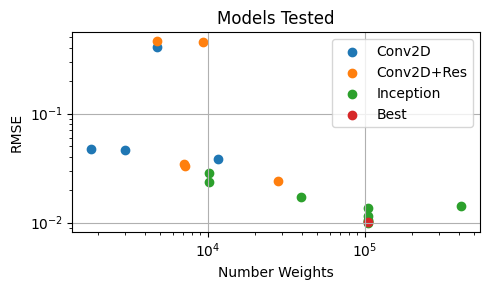
\includegraphics[width=0.95\columnwidth]{./fig/models.png}
        \caption{Resultados dos modelos testados por número de pesos.}\label{fig:modelos}
    \end{figure}

    \begin{table}
    \begin{center}
        \caption{Hiperparâmetros do modelo \emph{ótimo}.}
        \label{tab:hiperparam}
        \vspace{5pt}
        \begin{tabular}{c c}
            \toprule
            \textbf{Hiperparâmetro} & \textbf{Valor} \\
            \midrule
            Blocos intermediários & 8 \\
            Canais no espaço latente: & 64 \\
            \emph{Batch normalization} & Sim \\
            Ligação direta \emph{externa} & Sim \\
            Ligações diretas \emph{internas} & Sim \\
            Bloco Inception & Sim \\
            % Aumentar dados com log & Não \\
            % \addlinespace
            % Resolução dos dados & 5,5 \\
            Tamanho do \emph{batch} & 128 \\
            % Otimizador & Adam \\
            % Taxa de aprendizado inical & 0.01 \\
            \bottomrule
        \end{tabular}
    \end{center}
    \end{table}

    Para aumentar a capacidade de generalização do modelo \emph{ótimo}, o treinamento incluiu a variação da escala dos valores da matriz $\textbf{A}$ e do vetor $\textbf{b}$. A ordem de grandeza dos valores variou entre $0.1$ e $10$. Os valores do vetor $\textbf{y}$ foram mantidos na faixa [-2,2] para que a função de perda seja comparável entre as amostras. O treinamento atingiu o critério de parada após 304 épocas (Figura \ref{fig:loss}).

    \begin{figure}[hbt!]
        \centering
        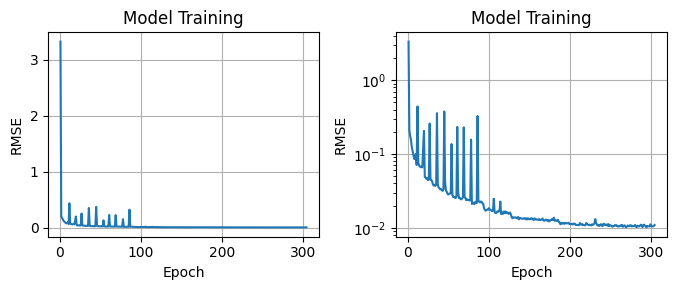
\includegraphics[width=0.95\columnwidth]{./fig/loss.png}
        \caption{Treinamento do modelo \emph{ótimo}.}\label{fig:loss}
    \end{figure}

    O treinamento do modelo foi realizado com amostras de malhas ($5,5$). Os resultados mostram que, mesmo que exista certa deteriorização da qualidade das respostas para malhas com outras configurações, o modelo conseguiu generalizar de modo satisfatório o problema proposto (Figura \ref{fig:rmse}). As figuras de \ref{fig:3x3} a \ref{fig:30x30} mostram exemplos de aplicação do modelo treinado\footnote{Exemplos com malhas maiores se encontram no repositório deste projeto: \href{https://github.com/TiagoCAAmorim/machine_learning/blob/main/Projeto/Relatorio/fig}{https://github.com/TiagoCAAmorim/machine\_learning/ blob/main/Projeto/Relatorio/fig}}. Os vetores $\textbf{y}_{exato}$ e $\textbf{y}_{modelo}$ são apresentados como uma série apenas para facilitar a visualização.

    \begin{figure}[hbt!]
        \centering
        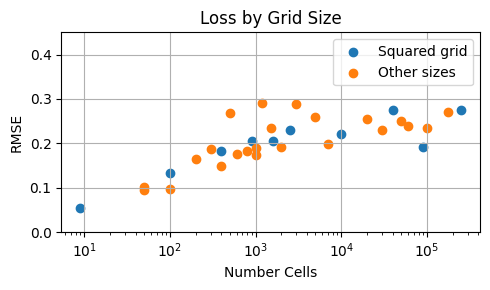
\includegraphics[width=0.85\columnwidth]{./fig/RMSE.png}
        \caption{Resultados do modelo \emph{ótimo} para diferentes tamanhos de malha.}\label{fig:rmse}
    \end{figure}

    \begin{figure}[hbt!]
        \centering
        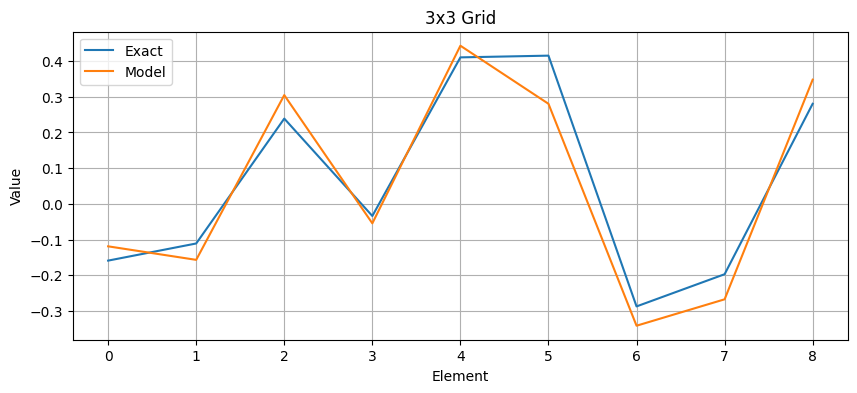
\includegraphics[width=0.85\columnwidth]{./fig/3x3.png}
        \caption{Exemplo de uma malha ($3$,$3$).}\label{fig:3x3}
    \end{figure}

    \begin{figure}[hbt!]
        \centering
        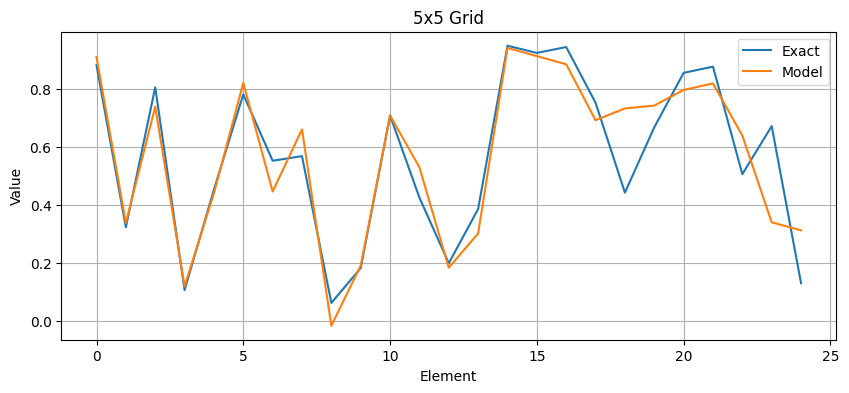
\includegraphics[width=0.85\columnwidth]{./fig/5x5.png}
        \caption{Exemplo de uma malha ($5$,$5$).}\label{fig:5x5}
    \end{figure}

    \begin{figure}[hbt!]
        \centering
        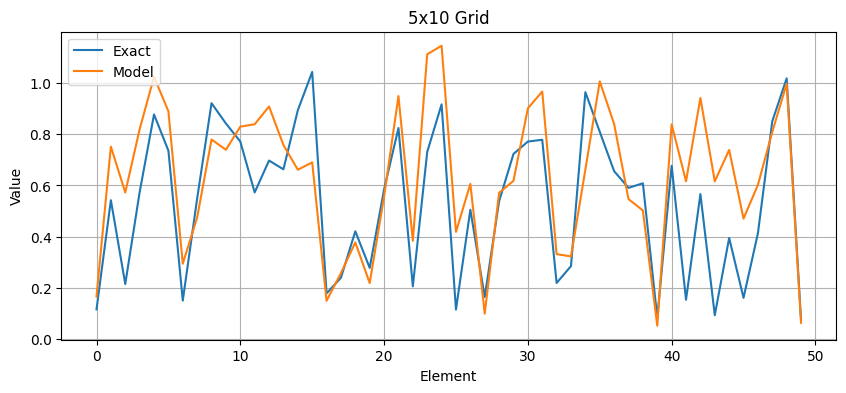
\includegraphics[width=0.85\columnwidth]{./fig/5x10.png}
        \caption{Exemplo de uma malha ($5$,$10$).}\label{fig:5x10}
    \end{figure}

    % \begin{figure}[hbt!]
    %     \centering
    %     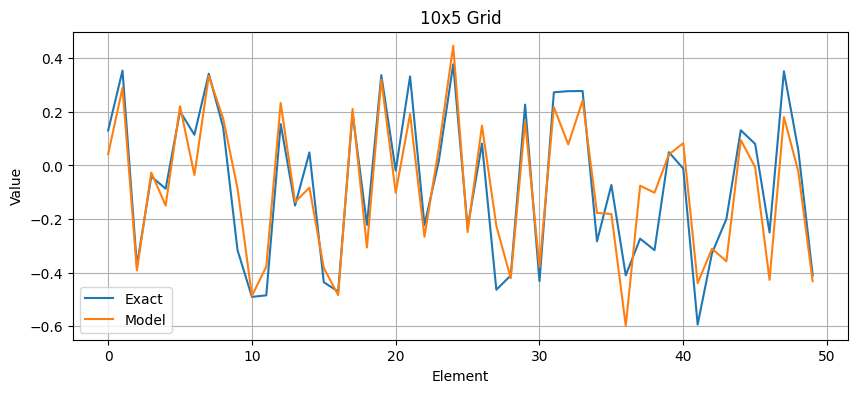
\includegraphics[width=0.95\columnwidth]{./fig/10x5.png}
    %     \caption{Exemplo de uma malha ($10$,$5$).}\label{fig:10x5}
    % \end{figure}

    \begin{figure}[hbt!]
        \centering
        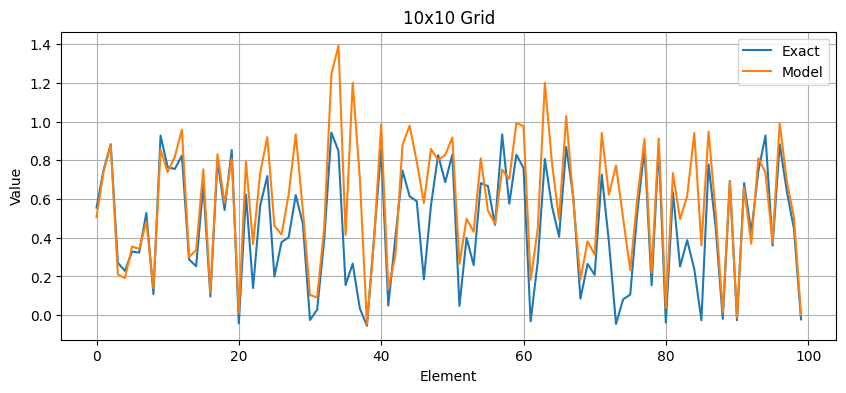
\includegraphics[width=0.85\columnwidth]{./fig/10x10.png}
        \caption{Exemplo de uma malha ($10$,$10$).}\label{fig:10x10}
    \end{figure}

    \begin{figure}[hbt!]
        \centering
        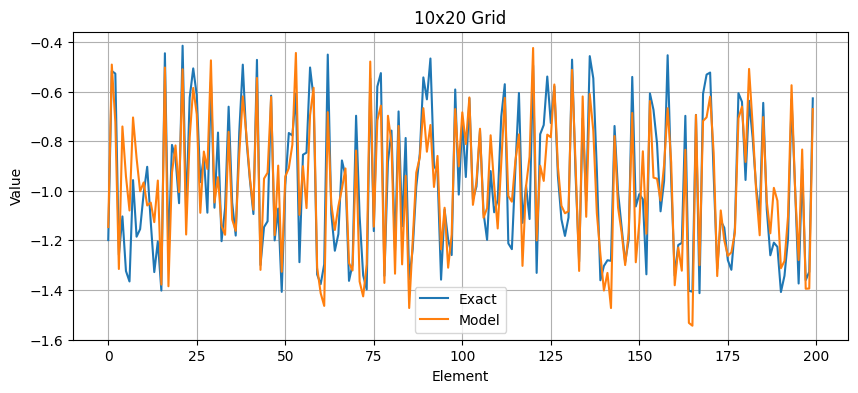
\includegraphics[width=0.85\columnwidth]{./fig/10x20.png}
        \caption{Exemplo de uma malha ($10$,$20$).}\label{fig:10x20}
    \end{figure}

    \begin{figure}[hbt!]
        \centering
        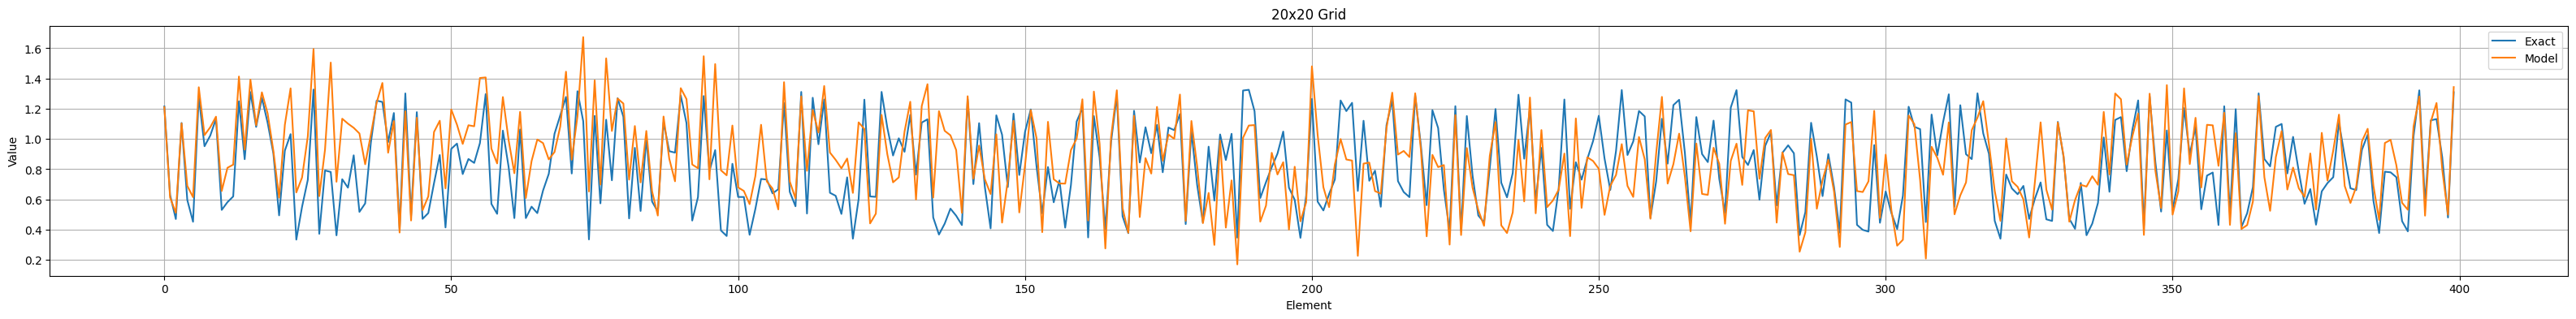
\includegraphics[width=0.95\columnwidth]{./fig/20x20.png}
        \caption{Exemplo de uma malha ($20$,$20$).}\label{fig:20x20}
    \end{figure}

    \begin{figure}[hbt!]
        \centering
        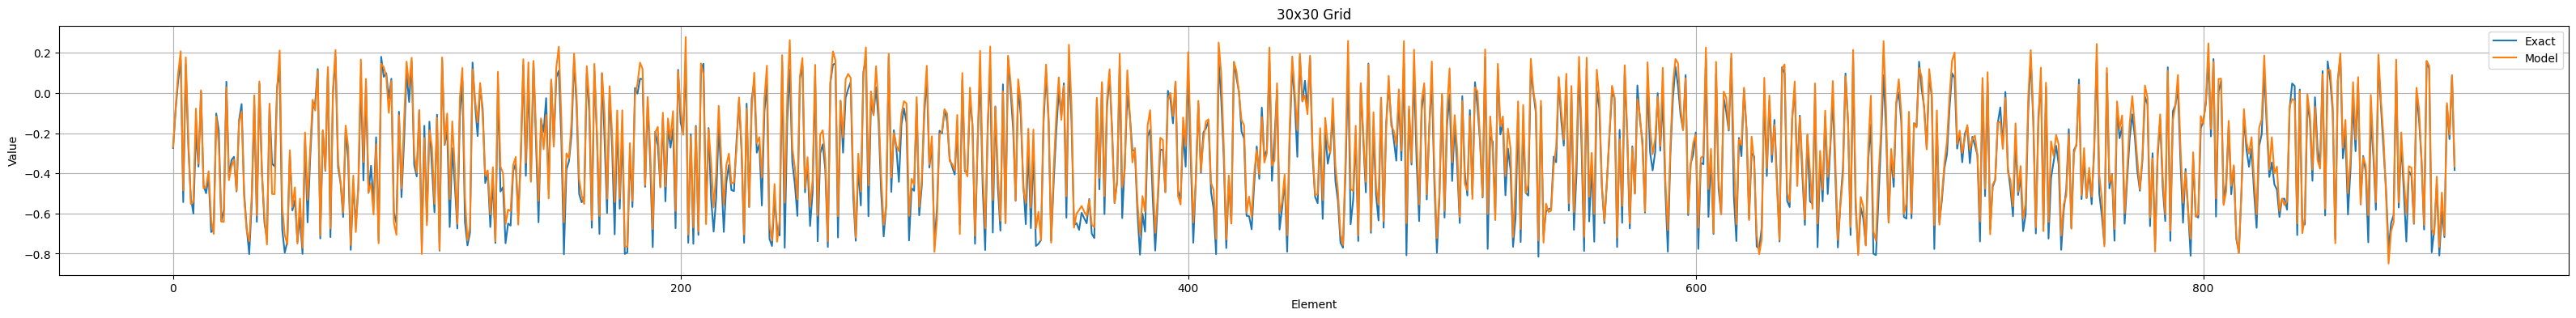
\includegraphics[width=0.95\columnwidth]{./fig/30x30.png}
        \caption{Exemplo de uma malha ($30$,$30$).}\label{fig:30x30}
    \end{figure}


    Todo o código foi desenvolvido em Pytorch, e está disponível em \href{https://github.com/TiagoCAAmorim/machine\_learning/blob/main/Projeto/solve_lin_eq.ipynb}{https://github.com/TiagoCAAmorim/machine \_learning/blob/main/Projeto/solve\_lin\_eq.ipynb}.


\section{Conclusões}

    A proposta inicial para este projeto foi de resolver um passo de tempo de uma simulação de fluxo em meio poroso. Esta tarefa se mostrou desafiadora, pois o que se espera da rede neural é que \emph{aprenda} a resolver um problema que da maneira tradicional envolve montar as matrizes de coeficientes a partir dos dados brutos do problema (porosidades, permeabilidades, viscosidades etc.) e resolver um sistema de equações não-lineares (usualmente por iteração, resolvendo vários sistemas lineares).

    O objetivo deste trabalho não foi o de propor uma nova abordagem para a solução de sistemas pentadiagonais. Existem algoritmos de alta performance que tratam deste tipo de problema \cite{levit1989parallel,ivanov1998parallel,carroll2021batched}. Neste trabalho buscou-se encontrar soluções para um problema mais simples que o inicialmente proposto, e aproveitar as lições aprendidas para a solução da proposta inicial, que será desenvolvida no futuro.

    O gráfico do treinamento do modelo \emph{ótimo} aponta para uma saturação da função de perda, que pode ser indicativo da falta de capacidade da própria rede neural de atingir melhores resultados. Testes com redes maiores tiveram problemas de convergência. Uma opção de trabalho futuro é treinar redes maiores a partir de redes menores já treinadas. Este mecanismo funciona como uma espécie de \emph{transfer learning}, em que as novas camadas irão ajudar a melhorar a resposta das camadas já treinadas.


% \appendix

%     \section{Redes Neurais Construídas}



%% \label{}

%% If you have bibdatabase file and want bibtex to generate the
%% bibitems, please use
%%

\bibliographystyle{elsarticle-num}
\bibliography{refs}

%% else use the following coding to input the bibitems directly in the
%% TeX file.

% \begin{thebibliography}{00}

%% \bibitem{label}
%% Text of bibliographic item

% \bibitem{}

% \end{thebibliography}


\end{document}
\endinput
